\documentclass[a4j,12pt,]{jarticle}
 \usepackage[dvipdfmx]{graphicx}
 \usepackage{float}
 \usepackage{siunitx} %%SI単位系用
 \usepackage{amssymb, amsmath}
 \usepackage{ascmac,here,txfonts,txfonts}
\usepackage{listings,jlisting}
\usepackage[dvipdfmx]{color}
\lstset{%
  language={Python},
  basicstyle={\small},%
  identifierstyle={\small},%
  commentstyle={\small\itshape\color[rgb]{0,0.5,0}},%
  keywordstyle={\small\bfseries\color[rgb]{0,0,1}},%
  ndkeywordstyle={\small},%
  stringstyle={\small\ttfamily\color[rgb]{1,0,1}},
  frame={tb},
  breaklines=true,
  columns=[l]{fullflexible},%
  numbers=left,%
  xrightmargin=0zw,%
  xleftmargin=3zw,%
  numberstyle={\scriptsize},%
  stepnumber=1,
  numbersep=1zw,%
  lineskip=-0.5ex%
}
\begin{document}

{\noindent\small 第7回報告書 \hfill\today}
\begin{center}
  {\Large 相互相関が最大となるラグの選定}
\end{center}
\begin{flushright}
  祖父江匠真 \\
\end{flushright}

\section{はじめに}
前回, 相互相関を用いて日時誤差が最小になるラグの選定を行ったが, 日時の間隔を全て均一にしなかったため, 正しい結果が得られなかった.
そこで今回は, 日時の間隔を均一になるよう線形補間した後に, 相互相関を用いて日時誤差が最小になるラグの選定を行う.

\section{実測値データの補間}
相互相関の計算を行う前に, 実測データの計測日時の間隔が均一でなかったため, 線形補間を行い, 日時間隔を1 \si{\second}に統一した.

\section{相互相関による最小ラグの選定}
相互相関の計算に使用する実測値の日射量データの範囲を, 2022年5月21日0時0分から2022年5月28日12時0分までの7.5日間とする.

次に, 計算値の日射量データの範囲を7日間として, 1分ずつスライドさせ, そのたびに実測値データとの相互相関を計算する.

今回, 計算値データを合計12時間(0.5日)スライドさせるため, Pythonでのリスト構造を用いた計算の都合を考えて, 合計スライド量の半分である6時間(0.25日)だけ計算値の日時データを進めた状態でスライドを開始する.

図\ref{p1}に, 上記の条件で計算した相互相関を示す.
横軸は, 実測値の日時と計算値の日時の差としている.

図\ref{p1}から, 計算値の日時を実測値より801秒進めた際に, 相互相関の値が最大となることが分かった.

\begin{figure}[H]
  \begin{center}
    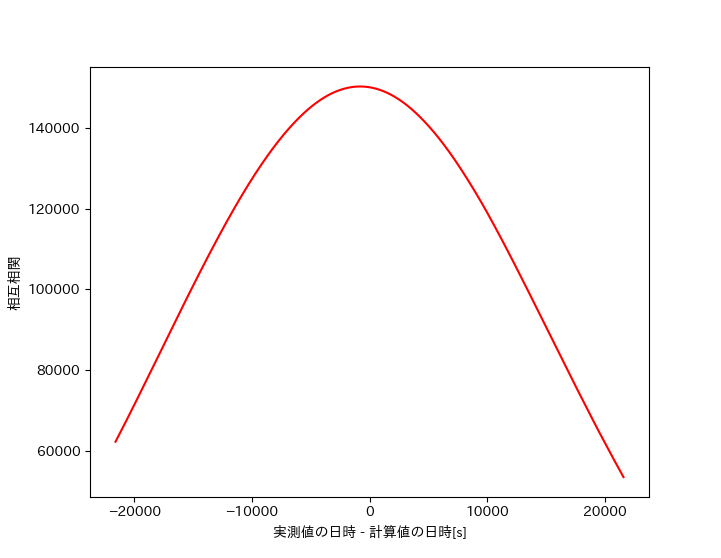
\includegraphics[width=160mm]{correlogram.png}
    \caption{相互相関}
    \label{p1}
  \end{center}
\end{figure}

\section{おわりに}
今回は, 日時の間隔を均一になるよう線形補間した後, 相互相関を用いて相互相関が最大となるラグの選定を行った.

\begin{thebibliography}{5}
  \bibitem{1}mattip, "numpy/numeric.py at v1.22.4 · numpy/numpy",\\ "https://github.com/numpy/numpy/blob/v1.22.4/numpy/core/numeric.py\#L670-L741", 参照 June 20, 2022.
\end{thebibliography}

\end{document}